\section{Introduction}

This chapter describe the methodology used to achieve statistically
sound comparisons of differing workgroup sizes on the performance of a
stencil code. I describe an experiment to explore the space of
architectures, programs, and datasets, and detail some of the many
factors which can influence the performance of stencils in different
conditions. I present the results of this exploration phase and use
this to present the case for autotuning.


\section{Defining the Optimisation Space}

This section describes the benchmarks, architectures, and datasets
used to gather performance data.


\subsection{Benchmark Stencil Applications}

To explore the effect of workgroup size across different stencils,
reference implementations of standard stencil applications from the
fields of image processing, cellular automata, and partial
differential equation solvers are used.

% \begin{table}
% \footnotesize
% \centering
% \begin{tabular}{| l | l | l | l | l |}
% \hline
% \textbf{Name} & \textbf{Application} & \textbf{Skeletons used} & \textbf{Iterative?} & \textbf{LOC}\\
% \hline
% CannyEdgeDetection & Image processing & Stencil & - & 225 / 61\\
% DotProduct & Linear algebra & Zip, Reduce & - & 143 / 2\\
% FDTD & Scientific simulation & Map, Stencil & Y & 375 / 127\\
% GameOfLife & Cellular automata & Stencil & Y & 92 / 12\\
% GaussianBlur & Image processing & Stencil & - & 262 / 47\\
% HeatSimulation & Scientific simulation & Stencil & Y & 180 / 13\\
% MandelbrotSet & Fractal computation & Map & Y & 133 / 78\\
% MatrixMultiply & Linear algebra & AllPairs & - & 267 / 8\\
% SAXPY & Linear algebra & Zip & - & 149 / 3\\
% \hline
% \end{tabular}
% \caption{Benchmark applications. The LOC column shows lines of code, split between host (C++) and device (OpenCL).}
% \label{tab:benchmarks}
% \end{table}

\TODO{Descriptions (with diagrams) for each application:}

\subsubsection{Finite Difference Time Domain}

\subsubsection{Heat Equation}

\subsubsection{Gaussian Blur}

The Gaussian blur is a common image processing algorithm, used to
reduce noise and detail in an image. A two dimensional Gaussian blur
defines a function to compute a pixel value $f(x,y)$ using a standard
deviation $\sigma$ using:

\begin{equation}
f(x,y) = \frac{1}{2\pi\sigma^2}e^{-\frac{x^2 + y^2}{2\sigma^2}}
\end{equation}

Gaussian blurs are parameterised by a radius $r$ which define
symmetric, square stencil regions about the centre
pixel. \TODO{Describe the range of blur radius' used.} Unlike the
previous two applications, a Gaussian blur is not iterative.

\subsubsection{Game of Life}

Conway's Game of Life (\FIXME{Citation needed}) is a cellular
automaton which models the evolution of a regular grid of cells over
discrete time steps. At each time step, each cell value is updated to
be either \emph{live} or \emph{dead} based on it's current value and
the value of the nearest neighbouring elements
(Algorithm~\ref{alg:gol}).

\begin{algorithm}[b]
\caption{Conway's Game of Life}
\label{alg:gol}
\begin{algorithmic}[1]
\Require current cell value $d_t$, neighbouring cell values $D_t$.
\Ensure new cell value $d_{t+1}$
\State $n \leftarrow $sum$(D_t)$
\If{$n = 3$ OR $(n = 2$ AND $d_t = 1)$}
  \State \textbf{return} 1
\Else
  \State \textbf{return} 0
\EndIf
\end{algorithmic}

\end{algorithm}

The stencil shape for Game of Life is always 1 in each direction.

\subsubsection{Canny Edge Detection}

The Canny edge detection algorithm consists of four distinct stages:
\TODO{4 separate stencils, with different behaviours.}


\subsection{Procedural Generation of Synthetic Stencils}

Synthetic benchmarks are a popular method for evaluating relative
performance of competing systems. The algorithmic generation of such
benchmarks has clear benefits for reducing evaluation costs; however,
creating meaningful benchmark programs is a difficult problem if we
are to avoid the problems of redundant computation and produce
provable halting benchmarks (\FIXME{Citations needed, although there
  will need to be a more extensive review of this in the related work
  chapter}).

In practise, stencil codes many common traits: a well tightly
constrained interface, predictable memory access patterns, and well
defined input and output data types. This can be used to create a
confined space of possible stencil codes by enforcing upper and lower
bounds on properties of the codes which can not normally be guaranteed
for general-purpose programs, e.g. the number of floating point
operations. By doing so, it is possible to create a system to
programatically generate synthetic stencil workloads which can .

One motivation for the use of synthetic benchmarks is that for the
purposes of autotuning, generating a large set of synthetic benchmarks
can address the ``small $n$, large $P$'' problem, which describes the
difficulty of statistical inference in spaces for which the set of
possible hypotheses $P$ is greatly larger than the number of
observations $n$\CitationNeeded. Creating parameterised, synthetic
benchmarks, it is possible to explore a much larger set of the space
of possible stencil codes than if relying solely on reference
applications, for example, to evaluate the performance impact of
highly irregular stencil shapes.

\FIXME{The synthetic benchmarks I've used aren't actually
  \emph{procedurally} generated. I'll either need to implement a
  system, or failing that, describe my method for creating the
  synthetic benchmarks and move the discussion of procedurally
  generated stencils into the future work section.}

The synthetic benchmarks used in this thesis are parameterised by
stencil shape (one parameter for each of the four directions), data
type (either integer or single or double precision floating point),
and \emph{complexity} a simple metric for indicating the desired
number of memory accesses and instructions per stencil.


\subsection{Selection of Parameter Values}

The parameter space is defined as the number of rows and columns in a
workgroup. To explore this 2D space, the following values are used in
each dimension: \input{gen/wg_c}. This provides a set of
\input{gen/num_params} possible combinations of workgroup size, e.g.\
$4 \times 4$, $4 \times 8$\ldots, $96 \times 96$. \TODO{Justify this
  choice of parameter values.}

% When exploring a non-uniform space such as the performance of
% workgroup sizes, there is a balance the cost of an exhaustive
% enumeration of the space with the risk of missing

The set of workgroup sizes which can be used for a specific program
and architecture is subject to two hard constraints: the maximum
workgroup size imposed by the architecture, and the maximum workgroup
size imposed by a kernel. Exceeding either of these constraints will
cause an \texttt{CL\_OUT\_OF\_RESOURCES} error when the OpenCL kernel
is enqueued.

\subsubsection{Architecture constraints}

Each OpenCL device imposes a maximum workgroup size which can be
statically checked by querying the \texttt{clGetDeviceInfo()}
API. These are defined by the limits of the hardware, typically the
number of execution units which have access to a shared memory pool.

\subsubsection{Kernel constraints}

At runtime, once an OpenCL program has been compiled to a kernel,
users can query the maximum workgroup size supported by that kernel
using the \texttt{clGetKernelInfo()} API. Crucially, this value cannot
be checked statically. That is, there is no way to determine the
maximum workgroup size for a given OpenCL source code and device
without first compiling it, which in OpenCL does not occur until
runtime. Factors which affect a kernel's maximum workgroup size
include the number registers required for a kernel, and the available
number of SIMD execution units for each type of instructions in a
kernel.


\section{Experimental Setup}

This section describes the environment under which performance data
was collected. Tables~\ref{tab:hw},~\ref{tab:kernels},
and~\ref{tab:datasets} list the range of execution devices, kernels,
and datasets used. For each unique combination of architecture,
kernel, and dataset (hereby referred to as a \emph{scenario}),
training data was collected by randomly sampling the space of legal
workgroup sizes, until multiple samples have been collected for each
combination of scenario and workgroup size.

\TODO{Description of each test system. E.g. mobo, memory, \& GPUs.}

\begin{table}
\scriptsize
\centering
\rowcolors{2}{white}{gray!25}
\begin{tabular}{ L{4.5cm} L{1.5cm} L{1.5cm} L{1.5cm} L{1.5cm} L{1.5cm} }
\hline
\scriptsize
\centering
\rowcolors{2}{white}{gray!25}
\begin{tabular}{ L{4.5cm} L{1.5cm} L{1.5cm} L{1.5cm} L{1.5cm} L{1.5cm} }
\hline
\scriptsize
\centering
\rowcolors{2}{white}{gray!25}
\begin{tabular}{ L{4.5cm} L{1.5cm} L{1.5cm} L{1.5cm} L{1.5cm} L{1.5cm} }
\hline
\input{gen/tables/devices}
\hline
\end{tabular}

\hline
\end{tabular}

\hline
\end{tabular}

\caption{%
  Execution devices. \FIXME{Missing data from CPUs!}%
}
\label{tab:hw}
\end{table}

\begin{table}
\scriptsize
\centering
\rowcolors{2}{white}{gray!25}
\begin{tabular}{lrrrrr}
\toprule
      Name &  North &  South &  East &  West &  Instruction Count \\
\midrule
   % complex &     30 &     30 &    30 &    30 &                161 \\
   % complex &      1 &     10 &    30 &    30 &                681 \\
   % complex &     20 &     10 &    20 &    10 &                161 \\
   % complex &      5 &      5 &     5 &     5 &                734 \\
   % complex &      5 &      5 &     5 &     5 &                161 \\
   % complex &      1 &     10 &    30 &    30 &                154 \\
   % complex &     10 &     10 &    10 &    10 &                161 \\
   % complex &     20 &     20 &    20 &    20 &                706 \\
   % complex &      1 &      1 &     1 &     1 &                137 \\
   % complex &     20 &     10 &    20 &    10 &                706 \\
   % complex &      1 &      1 &     1 &     1 &                661 \\
   % complex &     10 &     10 &    10 &    10 &                794 \\
   % complex &     30 &     30 &    30 &    30 &                706 \\
   % complex &     20 &     20 &    20 &    20 &                161 \\
   %  simple &      5 &      5 &     5 &     5 &                 67 \\
   %  simple &     20 &     10 &    20 &    10 &                612 \\
   %  simple &     20 &     20 &    20 &    20 &                612 \\
   %  simple &      1 &     10 &    30 &    30 &                592 \\
   %  simple &     10 &     10 &    10 &    10 &                700 \\
   %  simple &     30 &     30 &    30 &    30 &                612 \\
   %  simple &      1 &      1 &     1 &     1 &                 93 \\
   %  simple &     30 &     30 &    30 &    30 &                 67 \\
   %  simple &     20 &     10 &    20 &    10 &                 67 \\
   %  simple &      5 &      5 &     5 &     5 &                640 \\
   %  simple &     20 &     20 &    20 &    20 &                 67 \\
   %  simple &     10 &     10 &    10 &    10 &                 67 \\
   %  simple &      0 &      0 &     0 &     0 &                 40 \\
   %  simple &      1 &     10 &    30 &    30 &                 65 \\
   %  simple &      1 &      1 &     1 &     1 &                617 \\
   synthetic & 1--30 & 1--30 & 1--30 & 1--30 & 67--137\\
   synthetic & 1--30 & 1--30 & 1--30 & 1--30 & 592--706\\
   gaussian &      1--10 &      1--10 &     1--10 &     1--10 & 82--83 \\
  % gaussian &      5 &      5 &     5 &     5 &                655 \\
  % gaussian &      5 &      5 &     5 &     5 &                657 \\
  % gaussian &      0 &      0 &     0 &     0 &                 46 \\
  % gaussian &      5 &      5 &     5 &     5 &                 82 \\
  % gol &      1 &      1 &     1 &     1 &                714 \\
   gol &      1 &      1 &     1 &     1 &                190 \\
   he  &      1 &      1 &     1 &     1 &                113 \\
% he &      1 &      1 &     1 &     1 &                637 \\
%nms &      1 &      1 &     1 &     1 &                748 \\
   nms &      1 &      1 &     1 &     1 &                224 \\
%     sobel &      1 &      1 &     1 &     1 &               1008 \\
   sobel &      1 &      1 &     1 &     1 &                246 \\
% threshold &      0 &      0 &     0 &     0 &                 16 \\
   threshold &      0 &      0 &     0 &     0 &                 46 \\
\bottomrule
\end{tabular}

\caption{%
  Benchmark applications, border sizes, and static instruction counts.
  The ``simple'' and ``complex'' kernels are synthetic training
  programs. \FIXME{I also have a FDTD benchmark which I have yet to
    collect results for.}%
}
\label{tab:kernels}
\end{table}

\begin{table}
\footnotesize
\centering
\rowcolors{2}{white}{gray!25}
\begin{tabular}{ l l l l }
\hline
\footnotesize
\centering
\rowcolors{2}{white}{gray!25}
\begin{tabular}{ l l l l }
\hline
\footnotesize
\centering
\rowcolors{2}{white}{gray!25}
\begin{tabular}{ l l l l }
\hline
\input{gen/tables/datasets}
\hline
\end{tabular}

\hline
\end{tabular}

\hline
\end{tabular}

\caption{%
  Datasets used.%
}
\label{tab:datasets}
\end{table}


\subsection{Runtime Sampling and Statistical Soundness}

The number of ``moving parts'' in the modern software stack makes for
noisy results when measuring program execution time. As such,
evaluating the relative performance of different versions of programs
requires a judicious approach to isolate the appropriate performance
metrics and to take a statistically rigorous approach to collecting
data.


\subsubsection{Isolating the Impact of Workgroup Size}

The execution of a SkelCL stencil application can be divided into 6
distinct phases, shown in Table~\ref{tab:stencil-runtime-components}.

\TODO{Include a flow diagram}

\begin{table}
\footnotesize
\centering
\rowcolors{2}{white}{gray!25}
\begin{tabular}{ l l l l }
  \hline
  & \textbf{Description} & \textbf{Type} & \textbf{Cost}\\
  \hline
  $\bm{c}$ & Kernel compilation times & Host & Fixed \\
  $\bm{p}$ & Skeleton prepare times & Host & Fixed \\
  $\bm{u}$ & Host $\rightarrow$ Device transfers & Device & Fixed \\
  $\bm{k}$ & Kernel execution times & Device & Iterative \\
  $\bm{d}$ & Device $\rightarrow$ Host transfers & Device & Fixed \\
  $\bm{s}$ & Devices $\leftrightarrow$ Host (sync) transfers & Host & Iterative \\
  \hline
\end{tabular}

\caption{Execution phases of a SkelCL stencil skeleton. ``Fixed''
  costs are those which occur up to once per stencil
  invocation. ``Iterative'' costs are those which scale with the
  number of iterations of a stencil.}
\label{tab:stencil-runtime-components}
\end{table}

\paragraph{Kernel compilation times} Upon invocation, template
substitution is performed of the user code into the stencil skeleton
implementation, then compiled into an OpenCL program. Once compiled,
the program is cached for the lifetime of the host program.

\paragraph{Skeleton prepare times} Before a kernel is executed, a
preparation phase is required to allocate buffers for the input and
output data on each execution device.

\paragraph{Host $\rightarrow$ Device and Device $\rightarrow$ Host
  transfers} Data must be copied to and from the execution devices
before and after execution of the stencils, respectively. Note that
this is performed lazily, so iterative stencils do not require
repeated transfers between host and device memory.

\paragraph{Kernel execution times} This is the time elapsed executing
the stencil kernel, and is representative of ``work done''.

\paragraph{Devices $\leftrightarrow$ Host (sync) transfers} For
iterative stencils on multiple execution devices, an overlapping halo
region is shared at the border between the devices' grids. This must
be synchronised between iterations, requiring an intermediate transfer
to host memory, since device to device memory is not currently
supported by OpenCL.

For each of the six distinct phases of execution, accurate runtime
information can be gathered either through timers embedded in the host
code, or using the OpenCL \texttt{clGetEventProfilingInfo()} API for
operations on the execution devices. For single-device stencils, the
total time $t$ of a SkelCL stencil application is simply the sum of
all times recorded for each distinct phase:

\begin{equation}
t = \bm{1c} + \bm{1p} + \bm{1u} + \bm{1k} + \bm{1d}
\end{equation}

For multi-device stencils with $n$ execution devices, this can be
approximate as the sum of the sequential host-side phases, and the sum
of the device-side phases divided by the number of devices:

\begin{equation}
t \approx \sum_{i=1}^n{(\bm{1c}_{i})} + \bm{1p} + \bm{1s} +
  \frac{\sum_{i=1}^n{\bm{1u}_{i} + \bm{1k}_{i} + \bm{1d}_{i}}}{n}
\end{equation}

\TODO{Compare against empirical runtime information, showing how
  accurate this estimation is.}

The purpose of tuning workgroup size is to maximise the throughput of
stencil kernels. For this reason, isolating the kernel execution times
$\bm{k}$ produces the most accurate performance comparisons, as it
removes the impact of constant overheads introduced by memory
transfers between host and device memory, for which the selection of
workgroup size has no influence. Note that as demonstrated
in~\cite{Gregg2011}, care must be taken to ensure that isolating
device compute time does not cause misleading comparisons to be made
between across devices. For example, if using an autotuner to
determine whether execution of a given stencil is faster on a CPU or
GPU, the device transfer times $\bm{u}$, $\bm{d}$, and $\bm{s}$ would
need to be considered. For our purposes, we do not need to consider
the location of the data in the system's memory as it is has no
bearing on the throughput of a stencil kernel.


\subsubsection{Sampling plan and technique}

All runtimes were recorded with millisecond precision using either the
system clock or OpenCL's Profiling API. Measurement noise was
minimised by reducing system load through disabling all unwanted
services and graphical environments, and exclusive single-user access
was ensured for each machine. Frequency governors for each CPU were
disabled, and the benchmark processes were set to the highest priority
available to the task scheduler. Datasets and programs were stored in
an in-memory file system. A static sampling plan of 30 samples per
scenario was used.  \FIXME{Back this up with empirical data. Design
  and run an experiment to show how the choice of 30 samples is
  justified, or rather, why we can't get away with less.}

% Leather, H., O’Boyle, M., & Worton, B. (2009). Raced Profiles:
% Efficient Selection of Competing Compiler Optimizations. In LCTES
% ’09: Proceedings of the ACM SIGPLAN/SIGBED 2009 Conference on
% Languages, Compilers, and Tools for Embedded Systems
% (pp. 1–10). Dublin.
\TODO{%
  Consider using adaptive sampling plans to reduce the number of
  samples required to distinguish good from bad workgroup
  sizes~\cite{Leather2009}.%
}

\section{Results}

This section presents the results of the empirical enumeration of
workgroup size optimisation space for SkelCL stencils. A total of
\input{gen/num_runtime_stats} combinations of scenario and workgroup
size were tested, distributed across \input{gen/num_scenarios}
scenarios, with an average \input{gen/num_avg_params} unique workgroup
sizes each (max \input{gen/num_max_params}).

\subsection{Statistical soundness}

\begin{figure}
\centering
\includegraphics{gen/img/min_max_runtimes}
\caption{%
  Distribution of minimum and maximum observed runtimes for each
  combination of scenario and workgroup size, normalised to their
  respective mean runtimes. \FIXME{This is a weird way of getting the
    message across. Perhaps plot the distribution of all runtimes
    normalised to their respective mean?}%
}
\label{fig:min-max-runtimes}
\end{figure}

An average of \input{gen/avg_sample_count} runtimes were recorded per
scenario (total
\input{gen/num_samples}). Figure~\ref{fig:min-max-runtimes} shows the
distribution of minimum and maximum runtimes for each combination of
scenario and workgroup size. For a given scenario $s$ and workgroup
size $w$, the arithmetic mean of $n$ measured runtimes $\bar{t}$ is
calculated using:

\begin{equation}
\bar{t} = \frac{\sum_{i=1}^{n}t_i}{n}
\end{equation}

95\% confidence intervals are calculated assuming a Gaussian
distribution of runtimes (given our sample size of
$n \ge n$~\cite{Georges2007}):

\begin{align}
\sigma &= \sqrt{\frac{\sum_{i=1}^{n}(t_i - \bar{t})^2}{n - 1}}\\
c_1 &= \bar{t} - z_{1-\alpha/2}\frac{\sigma}{\sqrt{n}}\\
c_2 &= \bar{t} + z_{1-\alpha/2}\frac{\sigma}{\sqrt{n}}
\end{align}

\TODO{Actually demonstrate that differences in runtime between
  measured workgroup sizes are significant.}

\TODO{Plot variance of runtimes as a function of mean runtime.}

\subsection{Assessing Available Performance}

From the set of all workgroup sizes $W$, the subset of workgroup sizes
$W_{legal}(s) \subset W$ that are legal for a given scenario $s$ can
be found using:

\begin{equation}
W_{legal}(s) = \left\{w | w \in W, w < W_{max}(s) \right\}
\end{equation}

Where $W_{max}(s)$ is the maximum workgroup size constraints imposed
by the scenario device and kernel. Given a function $t(s,w)$ which
returns the arithmetic mean of the measured runtimes for a given
scenario $s$ and workgroup size $w$, we can calculate the speedup
$r(s, w_1, w_2)$ of competing workgroup sizes $w_1$ over $w_2$ using:

\begin{equation}
  r(s, w_1, w_2) = \frac{t(s,w_2)}{t(s,w_1)}\\
\end{equation}


\subsubsection{Oracle Workgroup Size}

For a given scenario, the \emph{oracle} workgroup size
$\Omega(s) \in W_{legal}(s)$ is the $w$ value which provided the
shortest average runtime. This allows for comparing the performance of
a particular workgroup against the maximum available performance for
that scenario:

\begin{align}
  \Omega(s) &= \argmin_{w \in W_{legal}(s)} t(s,w)\\
  p(s,w) &= r(s, w, \Omega(s))
\end{align}

Where the performance is within the range $0 \le p(s,w) \le 1$. For a
given workgroup size, the average performance $\bar{p}(w)$ across the
set of all scenarios $S$ can be found using the geometric mean of
performance relative to the oracle:

\begin{equation}
\bar{p}(w) =
\left(
  \prod_{s \in S} r(s, w, \Omega(s))
\right)^{1/|S|}
\end{equation}

The geometric mean is used to aggregate relative performances due to
it's multiplicative property~\cite{Fleming1986}.


\subsubsection{Performance Upper Bounds}

\begin{figure}
\begin{subfigure}[h]{\textwidth}
\centering
\includegraphics{gen/img/max_speedups.pdf}
\caption{%
  Worst workgroup size.%
}
\label{fig:oracle-speedups-worst}
\end{subfigure}
\\
\begin{subfigure}[h]{\textwidth}
\centering
\includegraphics{gen/img/oracle_speedups.pdf}
\caption{%
  Best static workgroup size.%
}
\label{fig:oracle-speedups-baseline}
\end{subfigure}

\caption{%
  Two comparisons of the performance of the best workgroup size for
  each scenario relative to: (\ref{fig:oracle-speedups-worst})~the
  worst workgroup size for each scenario; and
  (\ref{fig:oracle-speedups-baseline})~the workgroup size which
  provides the best average case performance across all scenarios.%
}
\label{fig:speedups}
\end{figure}

For a given scenario $s$, the ratio of the workgroups sizes from
$W_{legal}(s)$ which provide the longest and shortest mean runtimes
can be used to calculate the upper bound on the possible performance
improvements to be attained from selecting the workgroup size:

\begin{equation}
r_{max}(s) = r(s, \argmax_{w \in W_{legal}(s)} t(s,w), \Omega(s))
\end{equation}

When applied to each scenario $s \in S$ from the experimental results,
the range of performance upper bounds is found to be
$\input{gen/min_possible_speedup}\times$ -
$\input{gen/max_possible_speedup}\times$ (geometric mean
$\input{gen/avg_possible_speedup}\times$). Figure~\ref{fig:oracle-speedups-worst}
shows the maximum attainable speedups achieved for all scenarios.


\subsubsection{Establishing a Baseline}

By defining $W_{safe} \in W$ as the intersection of legal workgroup
sizes across all scenarios, the optimal \emph{static} workgroup size
$\bar{w}$ can be calculated as the workgroup size which provides which
provides the best average case performance:

\begin{align}
W_{safe} &= \cap \left\{ W_{legal}(s) | s \in S \right\}\\
\bar{w} &= \argmax_{w \in W_{safe}} \bar{p}(w)
\end{align}

From the experimental results, the baseline workgroup size $\bar{w}$
is \input{gen/one_r}, with a geometric mean performance
$\bar{p}(\bar{w})$ of
\input{gen/one_r_perf}. Figure~\ref{fig:oracle-speedups-baseline}
shows the average speedup of the oracle over this baseline for all
scenarios. If we assume that a pragmatic developer with enough time
would eventually find this static optimal, then this provides a
reasonable upper bound on the attainable improvements of an autotuner
for workgroup size over that of a static choice.


\subsection{Distribution of Oracle Workgroup Sizes}

\begin{figure}
\begin{subfigure}[t]{0.98\textwidth}
\centering
\includegraphics{gen/img/max_wgsizes.pdf}
\vspace{-1.5em} % Shrink vertical padding
\caption{}
\label{fig:max-wgsizes}
\end{subfigure}
\\
\begin{subfigure}[t]{0.98\textwidth}
\centering
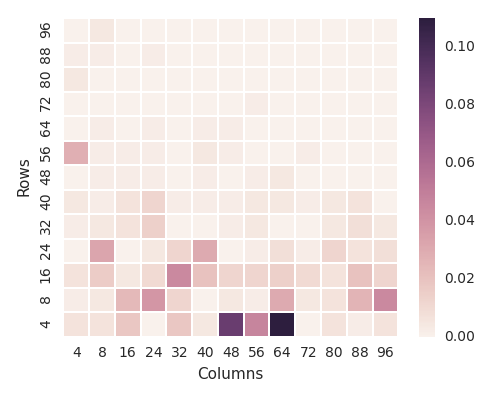
\includegraphics{gen/img/oracle_param_space.pdf}
\vspace{-1.5em} % Shrink vertical padding
\caption{}
\label{fig:oracle-wgsizes}
\end{subfigure}

\caption{%
  The distribution of: (\subref{fig:max-wgsizes}) maximum legal
  workgroup sizes, and (\subref{fig:oracle-wgsizes}) for all
  scenarios. The distribution of oracle workgroup sizes is uneven and
  spread across the space.%
}
\label{fig:heatmaps}
\end{figure}

Figure~\ref{fig:max-wgsizes} shows the distribution of maximum
workgroup sizes across all scenarios. Figure~\ref{fig:oracle-wgsizes}
shows the distribution of oracle workgroup sizes, demonstrating that
there is clearly no ``silver bullet'' workgroup size which works for
all scenarios. As Figure~\ref{fig:oracle-accuracy} shows,
\input{gen/num_wgsizes_50_accuracy} unique workgroup sizes are
required in order to achieve oracle performance just 50\% of the time.

\begin{figure}
\centering
\includegraphics{gen/img/num_params_oracle.png}
\caption{%
  Accuracy compared to the oracle as a function of the number of
  workgroup sizes used. The best accuracy that is achievable using a
  single statically chosen value is
  \protect\input{gen/max_oracle_param_frequency}.%
}
\label{fig:oracle-accuracy}
\end{figure}

The mode of the oracle workgroup sizes is
\input{gen/max_oracle_param}, which is optimal for
\input{gen/max_oracle_param_frequency} of scenarios. Note that this is
a different value from the \emph{baseline} identified previously,
which identifies the single choice which provides the best average
case performance. This is because the value is not legal for all
scenarios; that is, $\input{gen/max_oracle_param_w} \not\in W_{safe}$.
Figure~\ref{fig:performance-legality} illustrates this point by
plotting the geometric mean performance across workgroup sizes for:
all scenarios, and only the scenarios for which the workgroup size is
legal.

\begin{figure}
\centering
\includegraphics{gen/img/params_summary.png}
\caption{%
  The red line shows the ``legality'' of the parameter value, i.e.\
  the ratio of scenarios for which that workgroup size is legal.  The
  blue and green lines show the geometric mean of the performance of
  workgroup sizes relative to the oracle for: all scenarios, and only
  the scenarios for which the workgroup size is legal.%
}
\label{fig:performance-legality}
\end{figure}


\subsubsection{Factors Influencing Workgroup Size Performance}

A common approach taken by application developers is to set the
workgroup size for a kernel based on the maximum legal workgroup size,
for example to use the square root of the maximum to set the number of
columns and rows. While the reasoning for this approach is perfectly
intuitive, these results indicate that there no useful correlation
between the ratio of a particular workgroup size to the maximum legal
workgroup and the observed performance, as shown in
Figure~\ref{fig:performance-wgsizes}. Furthermore, the performance of
workgroup sizes is shown in Figure~\ref{fig:performances} to be vary
greatly across architectures, kernels, and datasets.

\TODO{Go into some detail here about the knock-on effect that changing
  workgroup size has on memory utilisation and execution unit
  occupancy.}

\begin{figure}
\begin{subfigure}[h]{\textwidth}
\centering
\includegraphics{gen/img/performance_max_wgsize}
\vspace{-1.5em} % Shrink vertical padding
\caption{}
\label{fig:performance-max-wgsize}
\end{subfigure}
\\
\begin{subfigure}[h]{.48\textwidth}
\centering
\includegraphics{gen/img/performance_max_c}
\vspace{-1.5em} % Shrink vertical padding
\caption{}
\label{fig:performance-wg-c}
\end{subfigure}
~%
\begin{subfigure}[h]{.48\textwidth}
\centering
\includegraphics{gen/img/performance_max_r}
\vspace{-1.5em} % Shrink vertical padding
\caption{}
\label{fig:performance-wg-r}
\end{subfigure}

\caption{%
  Comparing workgroup performance relative to the oracle as function
  of: (\subref{fig:performance-max-wgsize})~maximum legal size,
  (\subref{fig:performance-wg-c})~number of columns, and
  (\subref{fig:performance-wg-r})~ number of rows. As can be seen,
  workgroup size alone is not indicative of performance.%
}
\label{fig:performance-wgsizes}
\end{figure}

\begin{figure}
\begin{subfigure}[h]{\textwidth}
\centering
\includegraphics{gen/img/performance_kernels.pdf}
\vspace{-1.5em} % Shrink vertical padding
\caption{Kernels}
\label{fig:performance-kernels}
\end{subfigure}
\\
\begin{subfigure}[h]{.48\textwidth}
\centering
\includegraphics{gen/img/performance_devices.pdf}
\vspace{-1.5em} % Shrink vertical padding
\caption{Devices}
\label{fig:performance-devices}
\end{subfigure}
~%
\begin{subfigure}[h]{.48\textwidth}
\centering
\includegraphics{gen/img/performance_datasets.pdf}
\vspace{-1.5em} % Shrink vertical padding
\caption{Datasets}
\label{fig:performance-datasets}
\end{subfigure}

\caption{%
  Performance relative to the oracle of workgroup sizes across all
  scenarios, grouped by: (\subref{fig:performance-kernels})~kernels,
  (\subref{fig:performance-devices})~devices, and
  (\subref{fig:performance-datasets})~datasets.%
}
\label{fig:performances}
\end{figure}


\section{Summary}

The performance gap between different workgroup sizes can lead to
speedups of up to $\input{gen/max_possible_speedup}\times$.

\TODO{Hmm. It seems that there is a lot of room for improvement, which
demonstrates the problem with having to generalise for all cases - you
lose out on up to *10x* performance improvements. Let's put this all
together:}

\begin{enumerate}
\item The best workgroup size for a particular workload depends on the
  hardware, software, and dataset.
\item Not all workgroup sizes are legal, and we can only test if a
  value \emph{is} legal at runtime.
\item Differing workloads have wildly different optimal workgroup
  sizes, and selecting the right one can give you a 10x boost in
  performance.
\end{enumerate}

\todo{This presents a compelling case for the development of an
  autotuner which can select the optimal workgroup size at
  runtime. That is what I have set out to achieve.}
